\chapter{Introduzione}
\section{Terminologia di base}
Per avere un'implementazione corretta e completa del software dobbiamo fare 
in modo che il software risolva un problema concreto del mondo reale. Dobbiamo quindi 
comprendere correttamente il mondo reale, ovvero come funziona, come dovrebbe 
funzionare, quali sono i vincoli che governano, capire il contesto in cui il
software deve operare. Questo è il compito dell'ingegneria dei requisiti.

\begin{tcolorbox}[title=Esempio: il controllo di un'automobile]
\begin{itemize}
    \item \textbf{Problema}: la gestione del freno a mano in un'automobile 
    moderna potrebbe essere automatizzato.
    \item \textbf{Contesto}: se l'automobile è in movimento, 
    se si sta frenando, se è intenzione del guidatore fermarsi,
    se il guidatore ha premuto il pedale del freno, \dots
\end{itemize}
\end{tcolorbox}
Quando parliamo di \textbf{requisiti} dobbiamo inoltre definire il 
\textbf{mondo}. Quando definiamo il mondo, abbiamo a che fare con elementi molto 
complessi che contengono di fatto elementi umani (\textit{lo staff, 
l'utente, il cliente, \dots}), elementi fisici (\textit{dispositivi, 
software legacy, la natura, \dots}) e dovrà quindi adattarsi alla situazione 
esistente.

Dobbiamo definire anche il mondo delle \textbf{macchine}. Parliamo 
quindi di tutto ciò che dovrà essere implementato e/o acquistato, come ad esempio
\textit{database, server, client, \dots} e i componenti 
hardware e software che dovranno essere implementati.

L'ingegneria dei requisiti non si limita solamente al mondo delle 
macchine, ma tiene in considerazione anche gli effetti che il 
software ha sul mondo reale, che dovrà modellare. 

Il mondo e le macchine hanno i propri fenomeni, ma ne condividono 
anche alcuni. Ad esempio, il mondo ha il \textit{rilascio del freno a mano},
mentre le macchine hanno \texttt{errorCode = 013}. Nell'intersezione 
potremmo avere ad esempio \texttt{motor.Regime =`up`}.
\begin{figure}[H]
    \centering
    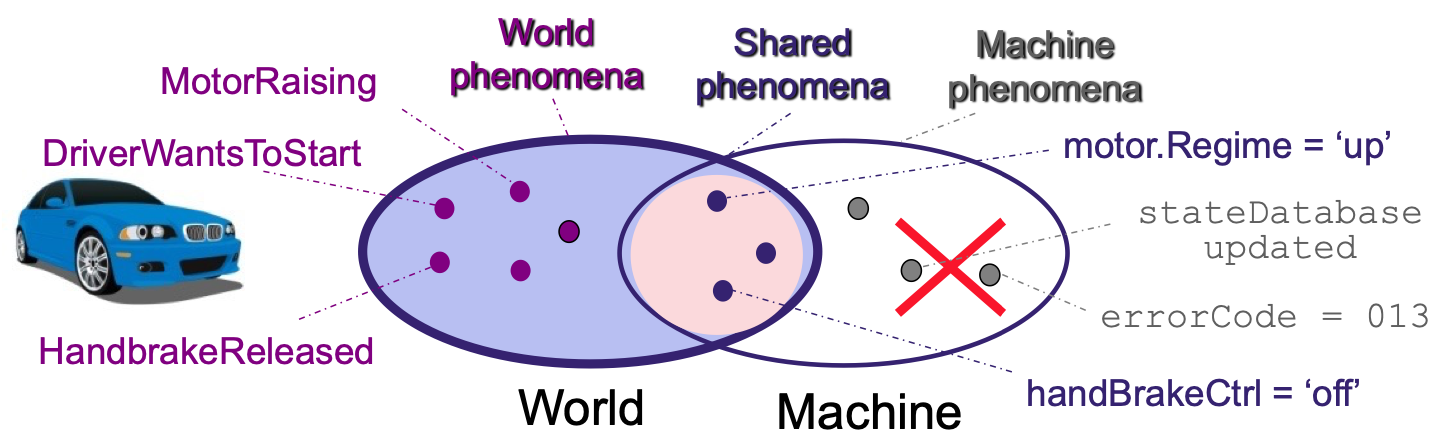
\includegraphics[scale=0.3]{img/worldmod.png}
    \caption{Il mondo e le macchine}
    \label{fig:req_eng}
\end{figure}
\begin{tcolorbox}
    Quando parliamo di requisiti, consideriamo solamente la parte 
    relativa al mondo, che comprende quindi anche l'intersezione.
    È importante comprendere che non descrivono \textbf{nulla}
    riguardo alle macchine.
\end{tcolorbox}
\subsection{Le due versioni del mondo}
Il sistema è l'insieme delle interazioni delle componenti che 
strutturano il mondo.
\begin{itemize}
    \item Il sistema \textbf{as-is}: si tratta del sistema prima che 
    il software venga implementato. Questo sistema è composto da
    solamente dal mondo.
    \item Il sistema \textbf{to-be}: si tratta del sistema come 
    dovrebbe essere quando il software opererà. Questo sistema
    è composto dall'unione del mondo e delle macchine.
\end{itemize}
\begin{tcolorbox}[title=Definizione preliminare dell'ingegneria dei requisiti]
    Consiste in una serie di attività collegate tra loro che ci permettono 
    di esplorare, valutare, documentare, consolidare, rivedere e adattare 
    quelli che sono gli obiettivi, le capacità, i vincoli e le assunzioni 
    in un sistema software. Basato sui problemi del sistema \textbf{as-is}
    e le opportunità date dalle nuove tecnologie.
\end{tcolorbox}

\subsection{I requisiti di sistema e i requisiti software}
Il sistema (\textit{unione del mondo reale e del sistema software}) sono 
i requisiti che fanno riferimento a tutto, si tratta degli statement che 
fanno parte del \textbf{system to-be}, mentre i requisiti software
sono un sottoinsieme dei requisiti di sistema, fanno quindi riferimento
solamente al \textbf{software to-be}, di fatto le funzionalità che il software 
che dovrà fornire per rispondere in maniera adeguata ai 
problemi del nostro utente.

\section{Scope dell'ingegneria dei requisiti}
\begin{figure}[H]
    \centering
    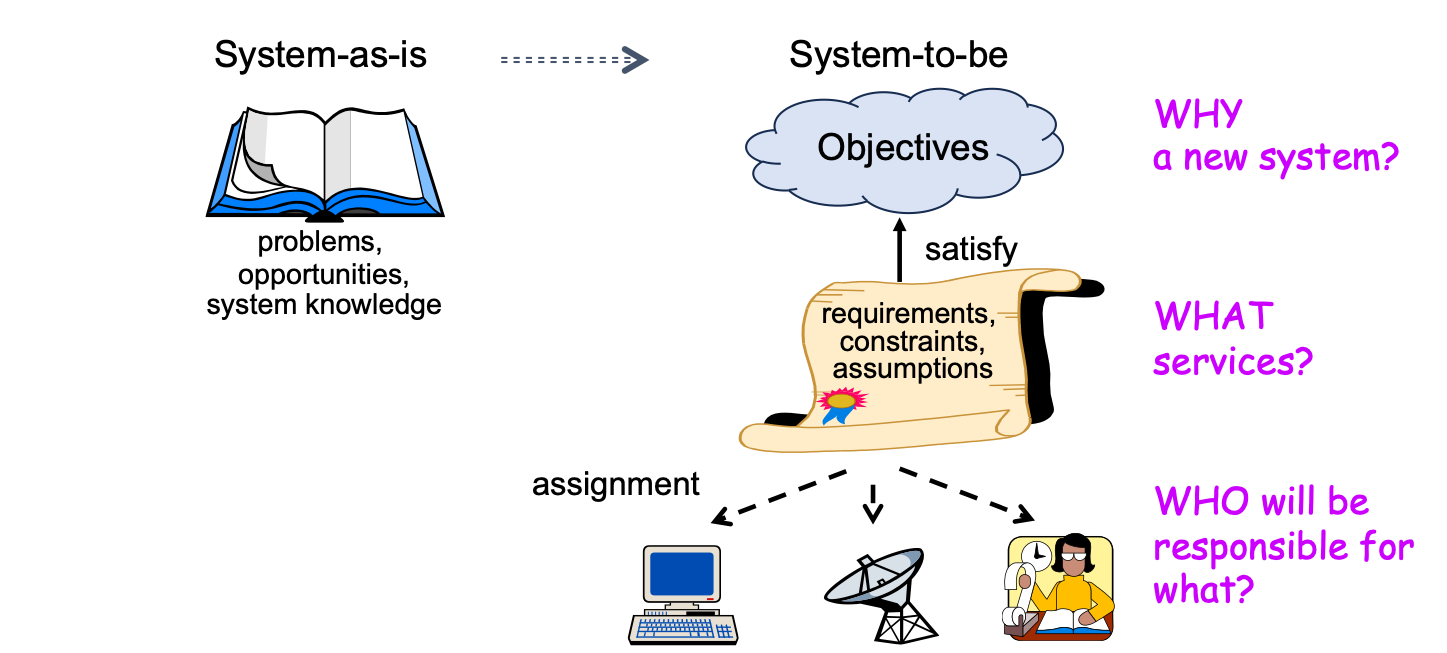
\includegraphics[scale=0.3]{img/scope.png}
    \caption{Scope dell'ingegneria dei requisiti}
    \label{fig:scope}
\end{figure}
Prima di iniziare a lavorare sui requisiti, abbiamo il nostro 
system as-is, che comprenderà i problemi, le opportunità e le 
conoscenze sul sistema. Da qui mapperemo il tutto nel 
system to-be. Per comprendere al meglio il system to-be,
dobbiamo ragionare in tre prospettive:
\begin{itemize}
    \item Perché: quali sono gli obiettivi dell'abbinamento 
    tra software e mondo reale. Quindi quali sono le necessità 
    che il software dovrà soddisfare.
    \item Cosa: quali sono le funzionalità che il software dovrà
    fornire per soddisfare i bisogni del cliente, quali saranno i 
    vincoli e le assunzioni che il software dovrà rispettare.
    \item Chi: chi sarà responsabile della fornitura 
    delle funzionalità.
\end{itemize}